% !Mode:: "TeX:UTF-8"
%% This is file `mcmthesis-demo.tex',
%% generated with the docstrip utility.
%%
%% The original source files were:
%%
%% mcmthesis.dtx  (with options: `demo')
%%
%% -----------------------------------
%%
%% This is a generated file.
%%
%% Copyright (C)
%%     2010 -- 2015 by Zhaoli Wang
%%     2014 -- 2015 by Liam Huang
%%
%% This work may be distributed and/or modified under the
%% conditions of the LaTeX Project Public License, either version 1.3
%% of this license or (at your option) any later version.
%% The latest version of this license is in
%%   http://www.latex-project.org/lppl.txt
%% and version 1.3 or later is part of all distributions of LaTeX
%% version 2005/12/01 or later.
%%
%% This work has the LPPL maintenance status `maintained'.
%%
%% The Current Maintainer of this work is Liam Huang.
%%
\documentclass{mcmthesis}
\mcmsetup{tcn = 46364, problem = C,
        sheet = true, titleinsheet = true, keywordsinsheet = false,
        titlepage = true, abstract = true}
%\usepackage{palatino}
\usepackage{times}

\usepackage{lipsum}
\renewcommand{\sfdefault}{ptm}
\title{A Nonlinear Programming Approach for the College Investment Problem}
\author{Zexiang Liu, Mingjian Fu, Yichang Gao}
\date{\today}


%\renewcommand\abstractname{Abstract}


\begin{document}
\begin{abstract}
\lipsum[1-2]

\begin{keywords}
keyword1; keyword2
\end{keywords}
\end{abstract}

\maketitle

%tocloft texdoc tocloft
\tableofcontents

\newpage

\section{Introduction}
<<<<<<< HEAD

\paragraph{} This article aims at proposing one model of the optimal investment strategy for the Goodgrant Foundation. The strategy will explicitly show the donated schools and their corresponding investment amount.This strategy results from the maximum return on the investment(ROI), which is an expectation for the positive effect on the student performance caused by the investment. It is obvious that this parameter is associated with not only the income improvement of the colleges and their graduates benefited from the investment, but also the social welfare. For example, the colleges should ensure the bottom amount for the minority students to promote racial equality. Another example is that the donation for the students from low income families should be keep to certain percentage because the investment can narrow the gap between the rich and poor. However, this kind of value cannot be indicated in any financial increase.
\paragraph{} According to the background, we hope to find the optimal strategy according to the following conditions.
\\ 	1. Maximize the return of the investment.
\\ 	2. Ensure the interests of some certain groups.
\paragraph{} Therefore, our team solves the problem in the following steps.
\\ 	1. Evaluate the effects of the variables in IPEDS data to the return of the investment.
\\  2. Construct the function of the total return for each school of the investment.
\\  3. Find the constraints of the investment amount considering students from certain social groups.
\\  4. Find the optimum solution of the function combining the  constraints.

=======
\paragraph{} This article aims at developing the model of the optimal investment strategy for the Goodgrant Foundation. The strategy will explicitly show the donated schools and their corresponding investment amount.This strategy results from the maximum "ROI" (return on that investment), which is an expectation for the positive effect on the student performance caused by the investment. It is obvious that this parameter is associated with not only the income improvement of the schools and their graduates benefited from the investment, but also the social welfare. For example, the colleges should ensure the bottom amount for the minority students to promote racial equality. Another example is that the donation for the students from low income families should be keep to certain percentage because the investment can narrow the gap between the rich and poor. However, this kind of value cannot be indicated in any financial increase.
\paragraph{} According to the background, we hope to find the optimal strategy according to the following conditions.
%\lipsum[2]
>>>>>>> 6eba5c1cad5f4f85a01543e53f6014fcf1870822
\begin{itemize}
\item Maximize the return of the investment.
\item Ensure the interests of some certain groups.
\end{itemize}
\paragraph{} Therefore, our team solves the problem in the following steps.

\begin{itemize}
\item Evaluate the effects of the variables in IPEDS data to the return of the investment.
\item Construct the function of the total return for each school of the investment.
\item Find the constraints of the investment amount considering students from certain social groups.
\item Find the optimum solution of the function combining the  constraints.
%\lipsum[3]
\end{itemize}
<<<<<<< HEAD

\begin{itemize}
\item the angular velocity of the bat,
\item the velocity of the ball, and
\item the position of impact along the bat.
\end{itemize}
\lipsum[4]
\emph{center of percussion} [Brody 1986], \lipsum[5]



%=======
\begin{Theorem} \label{thm:latex}
\LaTeX
\end{Theorem}
\begin{Lemma} \label{thm:tex}
\TeX .
\end{Lemma}
\begin{proof}
The proof of theorem.
\end{proof}


\section{Assumptions}

\paragraph{} 1. The investment only aims at the undergraduates.
\paragraph{} 2. The basic situation of these schools can be almost reflect from the provided data and, generally, the situation will not change.
\paragraph{} 3. The donation is only provided to the colleges whose scorecard data required is complete.
=======


%=======
%\begin{Theorem} \label{thm:latex}
%\LaTeX
%\end{Theorem}
%\begin{Lemma} \label{thm:tex}
%\TeX .
%\end{Lemma}
%\begin{proof}
%The proof of theorem.
%\end{proof}

\section{Assumptions}
\paragraph{} 1. The investment only aims at the undergraduates.
\paragraph{} 2. The basic situation of these schools can be almost reflect from the provided data and, generally, the situation will not change.
\paragraph{} 3. Performances of students in the same school are similar so that they can be assessed in a unified model.
\paragraph{} 4. The donation is only provided to the colleges whose scorecard data required is complete. 


\section{The Simplified Model}
\subsection{The yield of investment}  
\paragraph{} In order to find the optimal strategy, we compare the profit for each schools acquiring the donation. As the value qualifying the profit, a parameter is defined as $y$ (The yield of investment), which is a ratio of the average income of all the graduates and the roughly educational cost defined as $c$ of them at schools.This value is different for different schools to be the coefficient of the investment for each schools in the return function.
\paragraph{} We choose the "md\_earn\_wne\_p10" (Median earnings of students working and not enrolled 10 years after entry)defined as $p$ to be the standard of the average income of each students and the summation of "IPEDS"(Average net price for Title IV institutions (public institutions), the average annual total family cost of attendance) defined as $c_f$ and "GRAD\_DEBT\_MDN\_SUPP" (Median debt of completers) defined as $d$ to be the cost to provide education to each students in the college.

\begin{align}
y=\frac{p}{c}\\
c=c_f+d
\end{align}

\paragraph{} $y$ for all the potential candidate schools can be written as a vector $Y=(y_1, y_2, y_3, ..., y_N)$. Similarly, the investment for each schools can also be written as $X=(x_1, x_2, x_3, ..., x_N)$.

\subsection{The risk of investment}
\paragraph{} The investment is assumed to be the same amount of scholarship for every students in the school. However, some of the students cannot graduate from  the school for some reasons, the investment for whom is treated as being wasted. So the investment has its own risk. The risk can be reflected by the completion rate vector $R=(r_1, r_2, r_3, ..., r_N)$ which is "C150\_4\_POOLED\_SUPP" (150\% completion rate for four-year institutions, pooled in two-year rolling averages and suppressed for small n size.  For four year school, students are considered to have graduated "on time" if they graduate within 6 years.) or "C200\_L4\_POOLED\_SUPP" (200\% completion rate for less-than-four-year institutions, pooled in two-year rolling averages and suppressed for small n size.  For two year schools, students are considered to have graduated "on time" if they graduate within 4 years.). Therefore, the final $ROI$ function can be defined as:

\begin{align}
ROI=Y^T\*R^T\*X
\end{align}

\subsection{Preferential policies for some social groups}  
\paragraph{} Some constraints should also be developed such as the bottom line of the amount of donation for the minority students. We make a vector $M=(m_1, m_2, m_3, ..., m_N)$ whose elements is the minority students' rate of each potential candidate schools. The vector $N=(n_1, n_2, n_3, ..., n_N)$ indicates the number of students in each schools. So the constraint can be expressed as:
 
\begin{align}
M^T\*N^T\*X\geq\lambda_M\*\frac{M^T\*N}{I^T\*N}
\end{align}

\subparagraph{} ($\lambda_M$ is a coefficient to reflect the extent of the minority preferential treatment. $I$ is N dimensional unit vector.)
 
\paragraph{} The investment should also be distributed to all kinds of majors as fair as possible. We can find the data of percentage of degrees awarded in every schools ("PCIP01" to "PCIP54"). In the similar way, we divided the 54 majors of all the schools into Art, Science and Engineering, and define three vectors $A=(a_1, a_2, a_3, ..., a_N)$ for the percentage of Art degrees awarded in each schools. $S=(s_1, s_2, s_3, ..., s_N)$ for Science and $E=(e_1, e_2, e_3, ..., e_N)$ for Engineering. So the  major constraints can be expressed as:

\begin{align}
A^T\*N^T\*X\geq\lambda_A\*\frac{A^T\*N}{I^T\*N}\\
S^T\*N^T\*X\geq\lambda_S\*\frac{S^T\*N}{I^T\*N}\\
E^T\*N^T\*X\geq\lambda_E\*\frac{E^T\*N}{I^T\*N}\\
\end{align}

\subparagraph{} ($\lambda_A$, $\lambda_S$, $\lambda_E$ are coefficients to reflect the extent of the major being supported. $I$ is N dimensional unit vector.)
\paragraph{} With these constraints, we can find the solution $X$ for maximize the value of ROI function. The solution reflects the exact value of investment for each schools. 

\section{The advanced model} 
\paragraph{} In order to make the model more practical, we improve the design of the ROI function. In reality, the student performance will not be improved in a valid speed. Too little money may not be able to make any changes, but the proper amount of money for the student to keep in a best state of living and learning can develop his potential very well. Too much money can not even make better effect to the student.
\paragraph{} Therefore, we redesign the ROI function of each students profit rate of investment as an "S" curve, whose Horizontal coordinate is the investment amount per student and the vertical coordinate is the student's percentage. When the student get too little money, the performance change mildly. When getting proper amount of money, the student improve his performance swiftly. When he is over-donated, his performance change less and less and finally to his potential limit.

\begin{figure}
\centering
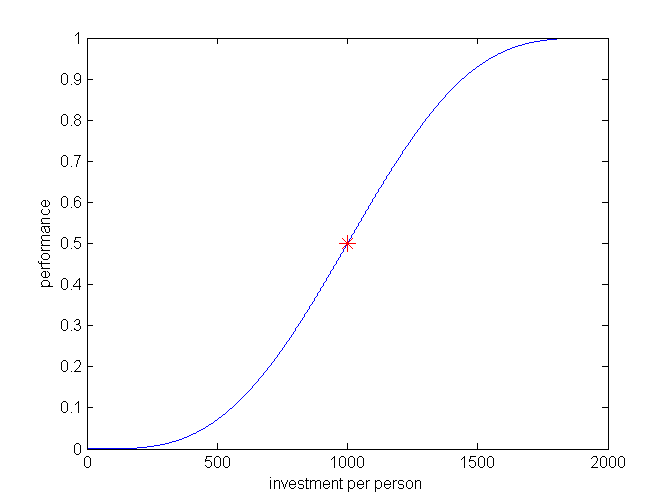
\includegraphics[width=0.5\textwidth]{sfun.png}
\caption{"S" curve}
\label{arch}
\end{figure}

\paragraph{} The "S" curve can be regarded as a graph of a function $f(x)=k\*\int_{0}^{x}(1-t^2)^3\*dt$ ($k$ is a coefficient.). We consider the curve starts from the origin. The coordinates of the point with max slope can be set as ($\mu, \frac{k}{2}$). The peak value of the "S" curve $k$ is the maximal potential a student can develop. It can be predicted by "md\_earn\_wne\_p10"$p$ (Median earnings of students working and not enrolled 10 years after entry).

\begin{align}
k=\*\lambda_p\*p
\end{align}

\subparagraph{} ($\lambda_p$ is a coefficient to qualify the student's potential.)

\paragraph{} $\mu$ is the most efficient amount of investment a student gets. The value of $\mu$ is related to the average private cost of students in the school. We think the For the reason that cost data is investigated in unit of school, every schools has its own $\mu$ for their students. 
\paragraph{} So the final function of 
>>>>>>> 6eba5c1cad5f4f85a01543e53f6014fcf1870822


\section{Analysis of the Problem}

%LaTeX插图指南
\begin{figure}[h]
\small
\centering
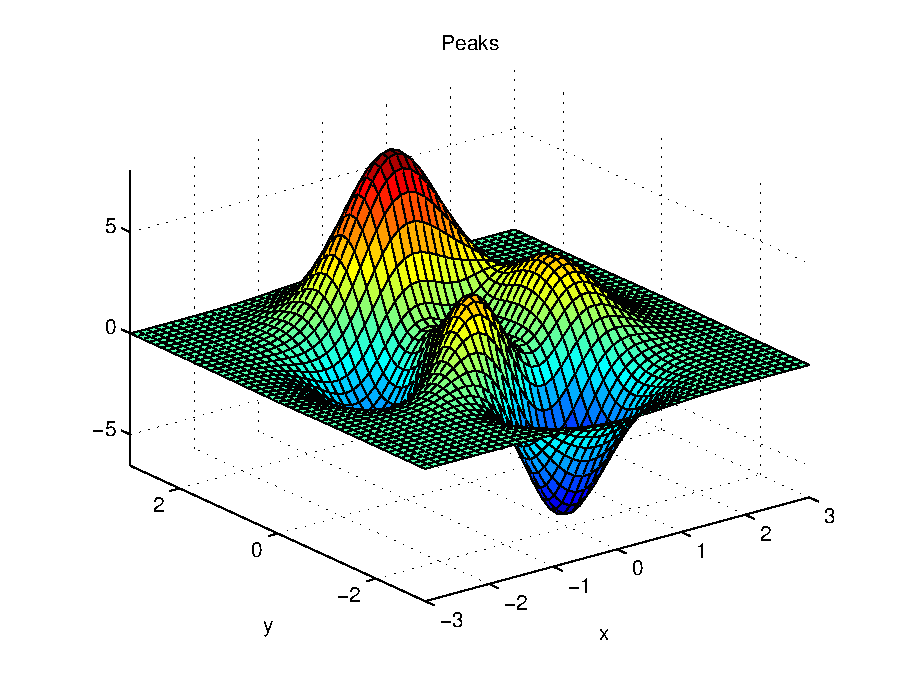
\includegraphics[width=12cm]{mcmthesis-aaa.eps}
\caption{aa} \label{fig:aa}
\end{figure}

%1,不要用子图,subfig,subfigure。
%2,尽量减少浮动环境,图尽量,缩小图的占位

\eqref{aa}
\begin{equation}
a^2 \label{aa}
\end{equation}

\[
  \begin{pmatrix}{*{20}c}
  {a_{11} } & {a_{12} } & {a_{13} }  \\
  {a_{21} } & {a_{22} } & {a_{23} }  \\
  {a_{31} } & {a_{32} } & {a_{33} }  \\
  \end{pmatrix}
  = \frac{{Opposite}}{{Hypotenuse}}\cos ^{ - 1} \theta \arcsin \theta
\]

\[
  p_{j}=\begin{cases} 0,&\text{if $j$ is odd}\\
  r!\,(-1)^{j/2},&\text{if $j$ is even}
  \end{cases}
\]

\[
  \arcsin \theta  =
  \mathop{{\int\!\!\!\!\!\int\!\!\!\!\!\int}\mkern-31.2mu
  \bigodot}\limits_\varphi
  {\mathop {\lim }\limits_{x \to \infty } \frac{{n!}}{{r!\left( {n - r}
  \right)!}}} \eqno (1)
\]

\section{Linear Model}

\subsection{The Model Results}

\section{Validating the Model}

\section{Conclusions}
\lipsum[6]

\section{A Summary}
\lipsum[6]

\section{Evaluate of the Mode}

\section{Strengths and weaknesses}
\lipsum[12]

\subsection{Strengths}
\begin{itemize}
\item \textbf{Applies widely}\\
This  system can be used for many types of airplanes, and it also
solves the interference during  the procedure of the boarding
airplane,as described above we can get to the  optimization
boarding time.We also know that all the service is automate.
\item \textbf{Improve the quality of the airport service}\\
Balancing the cost of the cost and the benefit, it will bring in
more convenient  for airport and passengers.It also saves many
human resources for the airline. 
\end{itemize}

%(author, 1998)  APA style.

\begin{thebibliography}{99}
\bibitem{1} D.~E. KNUTH   The \TeX{}book  the American
Mathematical Society and Addison-Wesley
Publishing Company , 1984-1986.
\bibitem{2}Lamport, Leslie,  \LaTeX{}: `` A Document Preparation System '',
Addison-Wesley Publishing Company, 1986.
\bibitem{3}\url{http://www.latexstudio.net/}
\bibitem{4}\url{http://www.chinatex.org/}
\end{thebibliography}

%\hspace{2em}
\begin{appendices}

\section{First appendix}

\lipsum[13]

Here are simulation programmes we used in our model as follow.\\

\textbf{\textcolor[rgb]{0.98,0.00,0.00}{Input matlab source:}}
\lstinputlisting[language=Matlab]{./code/mcmthesis-matlab1.m}

\section{Second appendix}

some more text \textcolor[rgb]{0.98,0.00,0.00}{\textbf{Input C++ source:}}
\lstinputlisting[language=C++]{./code/mcmthesis-sudoku.cpp}

\end{appendices}
\end{document}

%%
%% This work consists of these files mcmthesis.dtx,
%%                                   figures/ and
%%                                   code/,
%% and the derived files             mcmthesis.cls,
%%                                   mcmthesis-demo.tex,
%%                                   README,
%%                                   LICENSE,
%%                                   mcmthesis.pdf and
%%                                   mcmthesis-demo.pdf.
%%
%% End of file `mcmthesis-demo.tex'.
